\documentclass[11pt,letterpaper]{article}

\usepackage[margin=1in]{geometry}
\usepackage{amsmath,amssymb,amsthm}
\usepackage{enumitem}
\usepackage{hyperref}
\usepackage{booktabs}
\usepackage{fancyhdr}
\usepackage{listings}
\usepackage{xcolor}
\usepackage{tikz}
\usetikzlibrary{arrows.meta}

\newtheorem{theorem}{Theorem}
\newtheorem{lemma}[theorem]{Lemma}
\newtheorem{proposition}[theorem]{Proposition}
\theoremstyle{definition}
\newtheorem{definition}[theorem]{Definition}
\newtheorem{problem}{Problem}
\newtheorem{challenge}{Challenge}

\lstset{
  language=Python,
  basicstyle=\small\ttfamily,
  keywordstyle=\color{blue!70!black},
  commentstyle=\color{green!50!black},
  stringstyle=\color{red!60!black},
  showstringspaces=false,
  numbers=left,
  numberstyle=\tiny\color{gray},
  frame=single,
  breaklines=true,
  xleftmargin=2em,
  framexleftmargin=1.5em,
}

\pagestyle{fancy}
\fancyhf{}
\lhead{Tournament Enumeration Challenge}
\rhead{Algorithms \& High-Performance Computing}
\cfoot{\thepage}

\title{\vspace{-1.5em}\textbf{Tournament Enumeration Challenge} \\[6pt]
\large An exercise in algorithmic optimization \\[3pt]
\normalsize OEIS A000568: Non-isomorphic tournaments on $n$ vertices}
\author{Algorithms \& High-Performance Computing}
\date{}

\begin{document}
\maketitle
\thispagestyle{fancy}

\begin{quote}
\textit{``The formula has been known since 1954. The question is whether you can make it \emph{fast}.''}
\end{quote}

\vspace{-0.5em}

\section*{Background}

\begin{definition}
A \textbf{tournament} on $n$ vertices is a directed complete graph: for every pair of distinct vertices $\{u, v\}$, exactly one of the arcs $u \to v$ or $v \to u$ is present. Two tournaments are \textbf{isomorphic} if one can be obtained from the other by relabeling vertices.
\end{definition}

\begin{center}
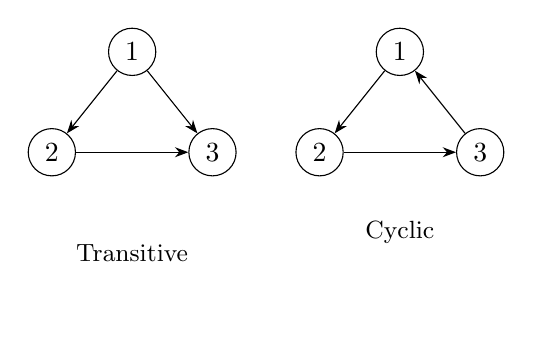
\begin{tikzpicture}[>=Stealth, every node/.style={circle, draw, minimum size=6mm, inner sep=1pt}, scale=0.85]
  % Tournament 1: transitive (1->2->3, 1->3)
  \node (a1) at (0, 1.5) {1};
  \node (a2) at (-1.2, 0) {2};
  \node (a3) at (1.2, 0) {3};
  \draw[->] (a1) -- (a2);
  \draw[->] (a2) -- (a3);
  \draw[->] (a1) -- (a3);
  \node[draw=none, below] at (0, -0.6) {\small Transitive};

  % Tournament 2: 3-cycle (1->2->3->1)
  \node (b1) at (4, 1.5) {1};
  \node (b2) at (2.8, 0) {2};
  \node (b3) at (5.2, 0) {3};
  \draw[->] (b1) -- (b2);
  \draw[->] (b2) -- (b3);
  \draw[->] (b3) -- (b1);
  \node[draw=none, below] at (4, -0.6) {\small Cyclic};
\end{tikzpicture}
\end{center}

\noindent The sequence $T(n)$ counting non-isomorphic tournaments on $n$ vertices is OEIS \href{https://oeis.org/A000568}{A000568}:
\[
1,\; 1,\; 1,\; 2,\; 4,\; 12,\; 56,\; 456,\; 6880,\; 191536,\; 9733056,\; \ldots
\]

\subsection*{History}

The exact formula for $T(n)$ was first published by \textbf{R.\ L.\ Davis} in 1954 (``Structure of dominance relations,'' \emph{Bull.\ Math.\ Biophys.}\ 16). It was independently derived by Frank Harary in 1957, and is a standard result in Harary \& Palmer's \emph{Graphical Enumeration} (1973). The formula is well-known, and implementations in Maple, PARI, Mathematica, and Python already exist on the OEIS page (by Jovovic 2001, Howroyd 2017, Alcover 2017, and Chai Wah Wu 2024, respectively).

\medskip
\noindent\textbf{This is not a mathematics problem --- it is a computer science problem.} The formula is given. Your challenge is to implement it efficiently enough to extend the OEIS, which lists $T(n)$ only up to $n = 76$ (77 terms, by Keith Briggs). How far and how fast can you go?

\bigskip
\hrule
\bigskip

%% ============================================================
%% PART 1: WARM-UP
%% ============================================================

\begin{problem}[\textbf{Warm-Up} --- 10 points]\label{prob:warmup}
\begin{enumerate}[label=(\alph*)]
  \item How many \emph{labeled} tournaments are there on $n$ vertices? Express your answer as a function of $n$.

  \item List all non-isomorphic tournaments on $n = 4$ vertices. For each one, give its \emph{score sequence} (the sorted list of out-degrees). Verify that $T(4) = 4$.

  \item One of the four $n = 4$ tournaments is \emph{self-complementary}: reversing every arc produces an isomorphic tournament. Which one?
\end{enumerate}
\end{problem}

\bigskip

%% ============================================================
%% PART 2: BRUTE FORCE
%% ============================================================

\begin{problem}[\textbf{Brute Force Baseline} --- 15 points]\label{prob:brute}
Write a program that computes $T(n)$ by \emph{exhaustive enumeration}:
\begin{enumerate}[label=(\alph*)]
  \item Generate all $2^{\binom{n}{2}}$ labeled tournaments on $n$ vertices.
  \item For each tournament, compute a \emph{canonical form} that is invariant under vertex relabeling. (One method: try all $n!$ permutations and take the lexicographic minimum.)
  \item Count the number of distinct canonical forms.
\end{enumerate}

\medskip
\noindent\textbf{Report:}
\begin{itemize}
  \item Verify $T(n) = 1, 1, 1, 2, 4, 12, 56, 456$ for $n = 0, \ldots, 7$.
  \item What is the largest $n$ your brute force handles in under 60 seconds?
  \item The complexity is $O(2^{\binom{n}{2}} \cdot n!)$. At $n = 10$ this is ${\sim}10^{20}$ operations. At $n = 100$ it is ${\sim}10^{1648}$. You need a fundamentally different approach.
\end{itemize}
\end{problem}

\bigskip

%% ============================================================
%% PART 3: THE FORMULA (given, not discovered)
%% ============================================================

\begin{problem}[\textbf{Implementing Davis's Formula} --- 30 points]\label{prob:formula}

The following formula is due to Davis (1954). We present it here; your job is to implement it.

\begin{theorem}[Davis's Formula for $T(n)$]\label{thm:davis}
\[
T(n) \;=\; \sum_{\substack{\lambda \vdash n \\ \text{all parts odd}}} \frac{2^{c(\lambda)}}{\displaystyle\prod_i l_i^{m_i} \cdot m_i!}
\]
where $\lambda = (l_1^{m_1}, l_2^{m_2}, \ldots)$ is a partition of $n$ written in exponential notation (part $l_i$ appears with multiplicity $m_i$), the sum runs only over partitions where every part $l_i$ is odd, and the \emph{cycle exponent} is:
\[
c(\lambda) \;=\; \sum_i m_i \left\lfloor \frac{l_i}{2} \right\rfloor + \sum_i \binom{m_i}{2} l_i + \sum_{i < j} m_i m_j \gcd(l_i, l_j).
\]
\end{theorem}

This comes from Burnside's lemma applied to the action of $S_n$ on tournaments. The ``all parts odd'' restriction is because permutations with any even-length cycle fix zero tournaments (the \emph{sign-flip constraint}: an even cycle forces contradictory arc orientations).

\medskip
\noindent For comparison, here is the formula as a Python one-liner, contributed to the OEIS by Chai Wah Wu (Jul 2024):

\begin{lstlisting}
from itertools import product
from math import prod, factorial, gcd
from fractions import Fraction
from sympy.utilities.iterables import partitions

def A000568(n):
    return int(sum(
        Fraction(
            1 << (sum(p[r]*p[s]*gcd(r,s)
                      for r,s in product(p.keys(), repeat=2))
                  - sum(p.values())) >> 1,
            prod(q**p[q] * factorial(p[q]) for q in p)
        )
        for p in partitions(n) if all(q & 1 for q in p)
    ))
\end{lstlisting}

\begin{enumerate}[label=(\alph*)]
  \item \textbf{Understand the formula.} Show that the exponent in Wu's one-liner,
  \[
  \frac{1}{2}\!\left[\sum_{r,s} m_r m_s \gcd(r,s) - \sum_r m_r\right],
  \]
  is algebraically equal to the cycle exponent $c(\lambda)$ from Theorem~\ref{thm:davis}. (Hint: expand the double sum into diagonal and off-diagonal terms.)

  \item \textbf{First implementation.} Translate the formula into a clean program (in any language). Verify against the known values in the table below. Report the time for $T(50)$.

  \begin{center}
  \begin{tabular}{c|rrrrrrrrrrr}
  \toprule
  $n$ & 0 & 1 & 2 & 3 & 4 & 5 & 6 & 7 & 8 & 9 & 10 \\
  \midrule
  $T(n)$ & 1 & 1 & 1 & 2 & 4 & 12 & 56 & 456 & 6880 & 191536 & 9733056 \\
  \bottomrule
  \end{tabular}
  \end{center}

  \item \textbf{Profile it.} Where does your program spend its time? What fraction is partition generation vs.\ the per-partition arithmetic? At what $n$ does it exceed 10 seconds?

  \item \textbf{The asymptotic formula.} Verify computationally that $T(n) \sim 2^{\binom{n}{2}} / n!$ as $n \to \infty$. At what $n$ does the ratio first exceed $0.999$? Explain in one sentence why the identity permutation dominates the Burnside sum.
\end{enumerate}
\end{problem}

\bigskip

%% ============================================================
%% PART 4: OPTIMIZATION
%% ============================================================

\begin{problem}[\textbf{Optimization} --- 30 points]\label{prob:optimize}

The na\"ive implementation of Davis's formula slows down around $n = 80\text{--}100$. Your task is to make it fast enough to compute $T(200)$.

\begin{enumerate}[label=(\alph*)]
  \item \textbf{GCD precomputation} (easy, ${\sim}1.5\times$).
  Build a lookup table $G[i][j] = \gcd(i,j)$ for $1 \leq i, j \leq n$ before the partition loop. Replace all \texttt{gcd()} calls with table lookups.

  \item \textbf{Avoid rational arithmetic} (medium, ${\sim}3\times$).
  The formula has a denominator $D(\lambda) = \prod l_i^{m_i} m_i!$ that varies per partition. Instead of using \texttt{Fraction} or dividing at each step:
  \begin{enumerate}[label=\roman*.]
    \item Compute $L = \mathrm{lcm}$ of all denominators $D(\lambda)$ across all partitions.
    \item For each partition, accumulate $(L / D(\lambda)) \cdot 2^{c(\lambda)}$ as an integer.
    \item Divide the total by $L$ once at the end.
  \end{enumerate}
  This replaces millions of GCD-based fraction reductions with one final division.

  \item \textbf{Bucket accumulation} (medium, ${\sim}3\text{--}5\times$).
  The values $2^{c(\lambda)}$ are enormous (up to $2^{19900}$ at $n = 200$). Instead of computing them per partition:
  \begin{enumerate}[label=\roman*.]
    \item Create an array \texttt{bucket[t]} indexed by the exponent $t = c(\lambda)$.
    \item For each partition, add $(L / D(\lambda))$ to \texttt{bucket[$c(\lambda)$]}.
    \item After the loop, compute $\sum_t \texttt{bucket}[t] \cdot 2^t$.
  \end{enumerate}
  This separates the expensive big-integer multiplications (one per distinct exponent value) from the cheap accumulation (one addition per partition).

  \item \textbf{Parallelization} (advanced, ${\sim}k\times$ for $k$ cores).
  The partition loop is embarrassingly parallel: each partition's contribution is independent. Describe (or implement) a strategy for splitting the work across threads. What data structure issues arise when multiple threads write to the same bucket array?

  \item \textbf{Language choice.} If using Python, compare your timings against a C or Rust implementation using GMP (GNU Multiple Precision Arithmetic). Report the speedup.
\end{enumerate}

\medskip
\noindent\textbf{Targets:}
\begin{center}
\begin{tabular}{lrl}
\toprule
Level & $n$ & Time target \\
\midrule
Bronze & 100 & $< 60$ seconds \\
Silver & 200 & $< 60$ seconds \\
Gold & 200 & $< 5$ seconds (compiled, multi-threaded) \\
\bottomrule
\end{tabular}
\end{center}
\end{problem}

\bigskip

%% ============================================================
%% PART 5: EXTEND THE OEIS
%% ============================================================

\begin{challenge}[\textbf{Extending the OEIS} --- Extra Credit]\label{chal:extend}

The OEIS b-file for A000568 contains 77 terms ($n = 0, \ldots, 76$), last updated by Keith Briggs.

\begin{enumerate}[label=(\alph*)]
  \item Compute $T(0)$ through $T(200)$ and format the output as an OEIS b-file.
  \item The same Burnside machinery computes other sequences by changing only the \texttt{edges()} function. Implement a \emph{unified enumerator} that computes any of the following from a single codebase:

  \begin{center}
  \begin{tabular}{llll}
  \toprule
  OEIS & Object & Constraint & OEIS terms \\
  \midrule
  A000568 & Tournaments & odd parts, base 2 & 77 \\
  A000088 & Simple graphs & all parts, base 2 & 95 \\
  A000273 & Directed graphs & all parts, base 2 & 65 \\
  A000595 & Binary relations & all parts, base 2 & 51 \\
  A001174 & Oriented graphs & all parts, base 3 & 50 \\
  A000665 & 3-uniform hypergraphs & all parts, base 2 & 29 \\
  A051240 & 4-uniform hypergraphs & all parts, base 2 & 19 \\
  \bottomrule
  \end{tabular}
  \end{center}

  Extend as many as you can beyond the current OEIS limits.
\end{enumerate}
\end{challenge}

\newpage

%% ============================================================
%% APPENDIX: HISTORY
%% ============================================================

\section*{Appendix A: Prior Art}

This formula is not new. Here is the chain of custody:

\begin{center}
\begin{tabular}{lll}
\toprule
Who & Year & Contribution \\
\midrule
R.\ L.\ Davis & 1954 & Original derivation of the partition formula \\
F.\ Harary & 1957 & Independent derivation via P\'olya enumeration \\
J.\ W.\ Moon & 1968 & Textbook treatment (\emph{Topics on Tournaments}, p.\ 87) \\
Harary \& Palmer & 1973 & Definitive reference (\emph{Graphical Enumeration}, pp.\ 126, 245) \\
B.\ Alspach & 1970 & Proved tournament automorphism groups have odd order \\
V.\ Jovovic & 2001 & Maple implementation, corrected Harary--Palmer errors \\
A.\ Howroyd & 2017 & Clean PARI implementation \\
J.-F.\ Alcover & 2017 & Mathematica translation \\
K.\ Briggs & pre-2007 & OEIS b-file to $n = 76$ \\
C.\ W.\ Wu & 2024 & Python one-liner (the code in Problem~\ref{prob:formula}) \\
\bottomrule
\end{tabular}
\end{center}

\noindent The mathematical content is 70 years old. The open problem is purely computational: no one has published terms beyond $n = 76$, because the na\"ive implementations slow down and the optimizations (LCD scaling, bucket accumulation, GMP arithmetic, parallelization) have not been applied to this problem in the literature. The barrier is engineering, not mathematics.

\section*{Appendix B: Reference Values}

{\small
\begin{center}
\begin{tabular}{r|r}
\toprule
$n$ & $T(n)$ \\
\midrule
0 & 1 \\
1 & 1 \\
2 & 1 \\
3 & 2 \\
4 & 4 \\
5 & 12 \\
6 & 56 \\
7 & 456 \\
8 & 6{,}880 \\
9 & 191{,}536 \\
10 & 9{,}733{,}056 \\
11 & 903{,}753{,}248 \\
12 & 154{,}108{,}311{,}168 \\
13 & 48{,}542{,}114{,}686{,}912 \\
14 & 28{,}401{,}832{,}763{,}013{,}120 \\
15 & 30{,}985{,}706{,}320{,}654{,}949{,}376 \\
\bottomrule
\end{tabular}
\end{center}
}

\medskip
\noindent At $n = 100$, $T(100)$ has 306 digits. At $n = 200$, it has 1{,}188 digits.

\vfill
\begin{center}
\small\itshape
``The formula is on the board. Make it fast.''
\end{center}

\end{document}
